\documentclass[12pt]{article}
\usepackage[utf8]{inputenc}
\usepackage[greek,english]{babel}
\usepackage{alphabeta}
\usepackage{fancyhdr}
\usepackage{listings}
\usepackage{mathtools}
\usepackage{xcolor}
\usepackage{float}
\usepackage{siunitx}
\usepackage[margin=0.5in]{geometry}
\usepackage[backend=bibtex]{biblatex}

\title{Εργαστήριο Μικροηλεκτρονικής -- Εργασία 4}
\author{Χρήστος Μαργιώλης -- 19390133}
\date{Ιούνιος 2022}

\begin{document}

\begin{titlepage}
        \maketitle
        \begin{figure}[t!]
        \begin{center}
        
\includegraphics[scale=0.3]{./res/uniwalogo.png} \\
        \Large
        \textbf{Πανεπιστήμιο Δυτικής Αττικής} \\
        \large
        Τμήμα Μηχανικών Πληροφορικής και Ηλεκτρονικών Υπολογιστών
        \end{center}
        \end{figure}
\end{titlepage}

\renewcommand{\contentsname}{Περιεχόμενα}
\tableofcontents
\pagebreak

\section{Θεωρητικό μέρος}

Το αντικείμενο της εργασίας είναι η εξοικείωση και η υλοποίηση ενός διαφοριστή.
Ο διαφοριστής είναι ένα κύκλωμα το οποίο εκτελεί την μαθηματική πράξη της
παραγώγησης σε ένα σήμα. 'Οσον αφορά το κύκλωμα, ο ιδανικός διαφοριστής είναι
ένας αναστρέφων Τ.Ε με την διαφορά ότι αντί για αντίσταση εισόδου υπάρχει
πυκνωτής ο οποίος έχει άεργη αντίσταση εισόδου. Στον πρακτικό διαφοριστή,
προκειμένου να περιορίσουμε το κέρδος του, προσθέτουμε και μία αντίσταση
εισόδου σε σειρά με τον πυκνωτή. Τέλος, για συχνότητα μεγαλύτερης της $F_c$, ο
διαφοριστής παύει να διαφορίζει και συμπεριφέρεται σαν απλός αναστρέφων Τ.Ε.

\section{Υλοποίηση της εργασίας}

Για την υλοποίηση της εργασίας χρησιμοποιήθηκαν τα παρακάτω εργαλεία:
\begin{itemize}
	\item Tina-TI για την συνδεσμολογία και τις μετρήσεις του κυκλώματος.
	\item Το breadboard του εργαστηρίου.
	\item \LaTeX για την συγγραφή της εργασίας.
\end{itemize}

\section{Συνδεσμολόγηση κυκλώματος}

\begin{itemize}
	\item Συνδεσμολογήστε το κύκλωμα με $R_{in} = \SI{2.2}{\kohm}$,
		$R_f = \SI{22}{\kohm}$, $C_1 = \SI{4.7}{\nano\farad}$,
		$V_1 = \SI{15}{\volt}$, $V_2 = \SI{-15}{\volt}$
\end{itemize}

\begin{figure}[H]
	\centering
	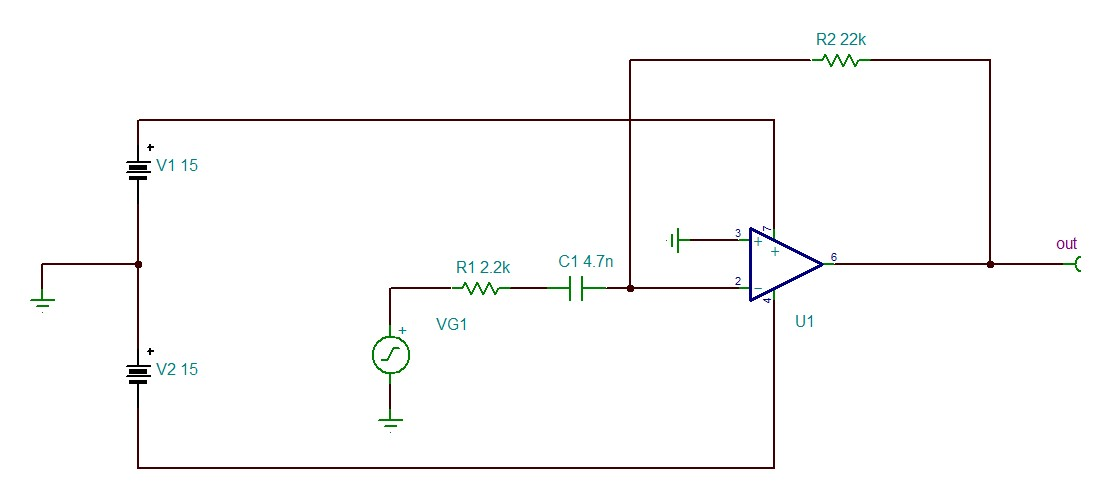
\includegraphics[width=\linewidth]{./res/schem.jpg}
	\caption{Διαφοριστής.}
\end{figure}

\section{Εφαρμογή σήματος}

\begin{itemize}
	\item Εφαρμόστε τριγωνική/ημιτονική/τετραγωνική κυματομορφή πλάτους
		$10V_{pp}$, $\SI{400}{\hertz}$ στην είσοδο του κυκλώματος.
\end{itemize}

\subsection{Θεωρητική $F_c$}

\begin{itemize}
	\item Υπολογίστε την θεωρητική $F_c$ του κυκλώματος.
\end{itemize}

\[F_c = \frac{1}{2 \pi R_{in} C} \Rightarrow
F_c = \frac{1}{2 \pi \cdot \SI{2.2}{\kohm} \cdot \SI{4.7}{\nano\farad}} \Rightarrow
F_c = \approx \SI{154000}{\hertz} \Rightarrow
F_c = \approx \SI{154}{\kilo\hertz}\]

\subsection{Γράφημα εξόδου}

\begin{itemize}
	\item Αναπαραστήστε σε γράφημα την έξοδο του κυκλώματος ως προς την
		είσοδο για $F = \SI{400}{\hertz}$, $F >> F_c$, $F << F_c$.
\end{itemize}

\begin{figure}[H]
	\centering
	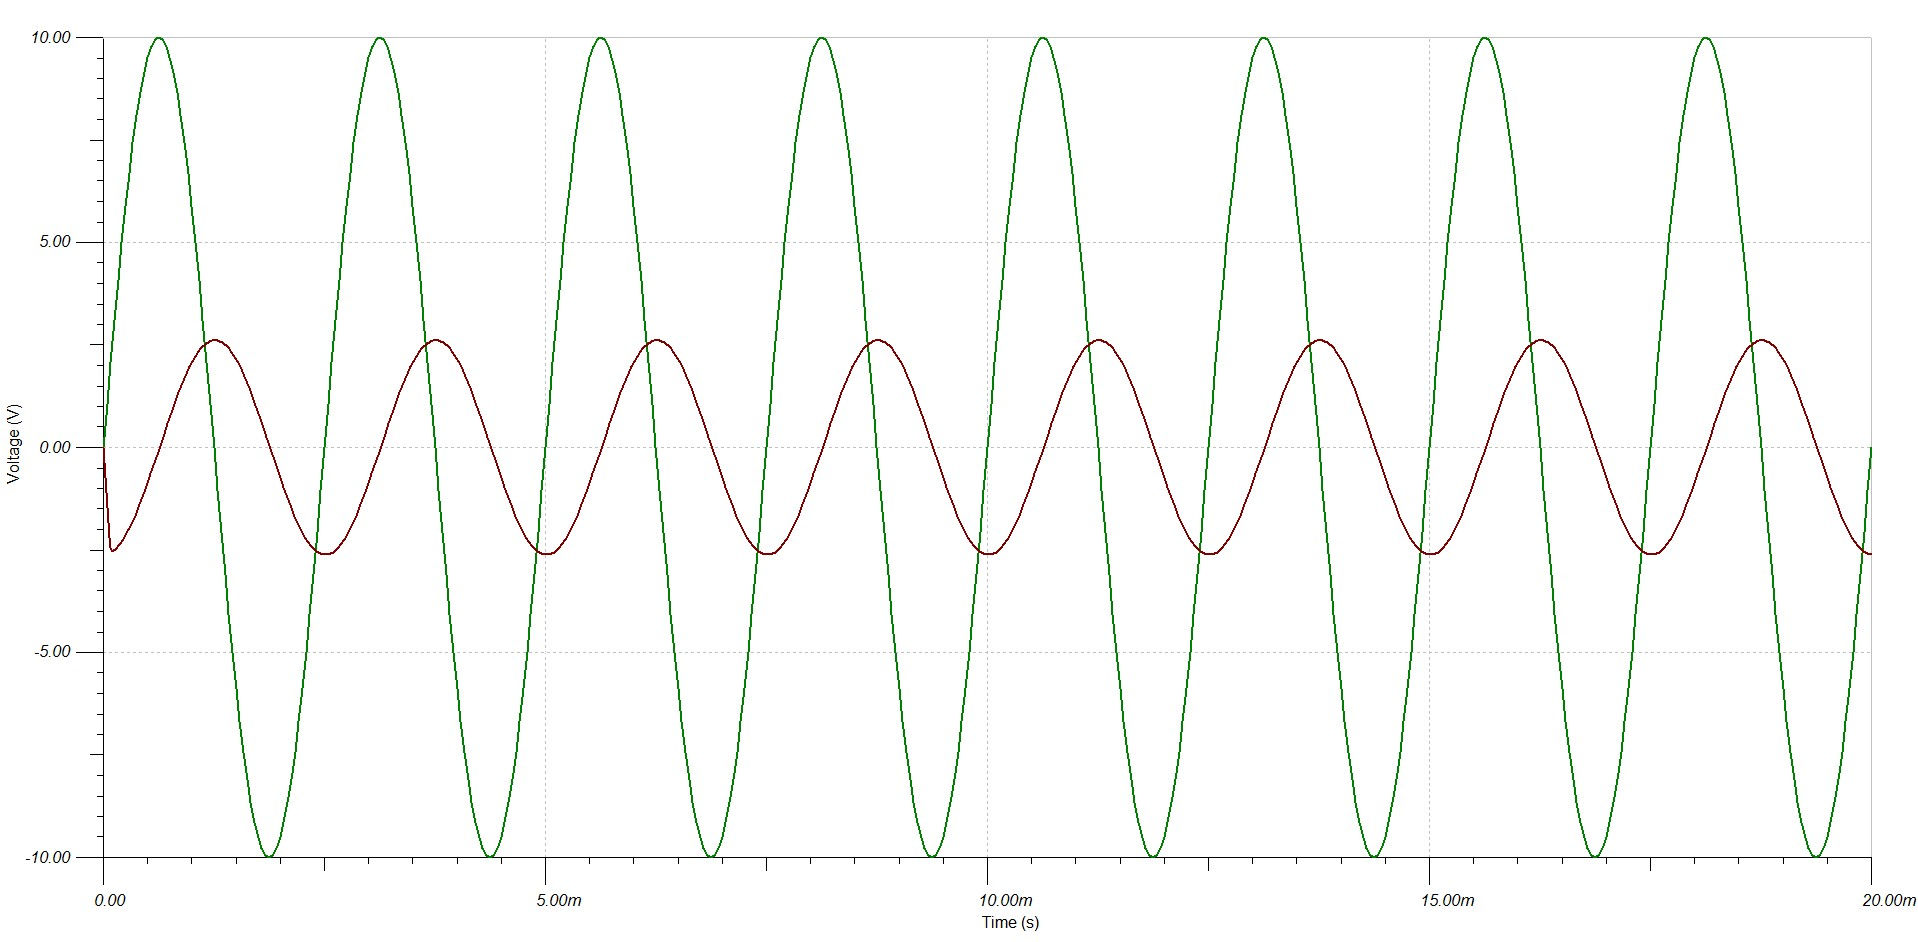
\includegraphics[width=\linewidth]{./res/sine.jpg}
	\caption{Ημιτονικό σήμα.}
\end{figure}

\begin{figure}[H]
	\centering
	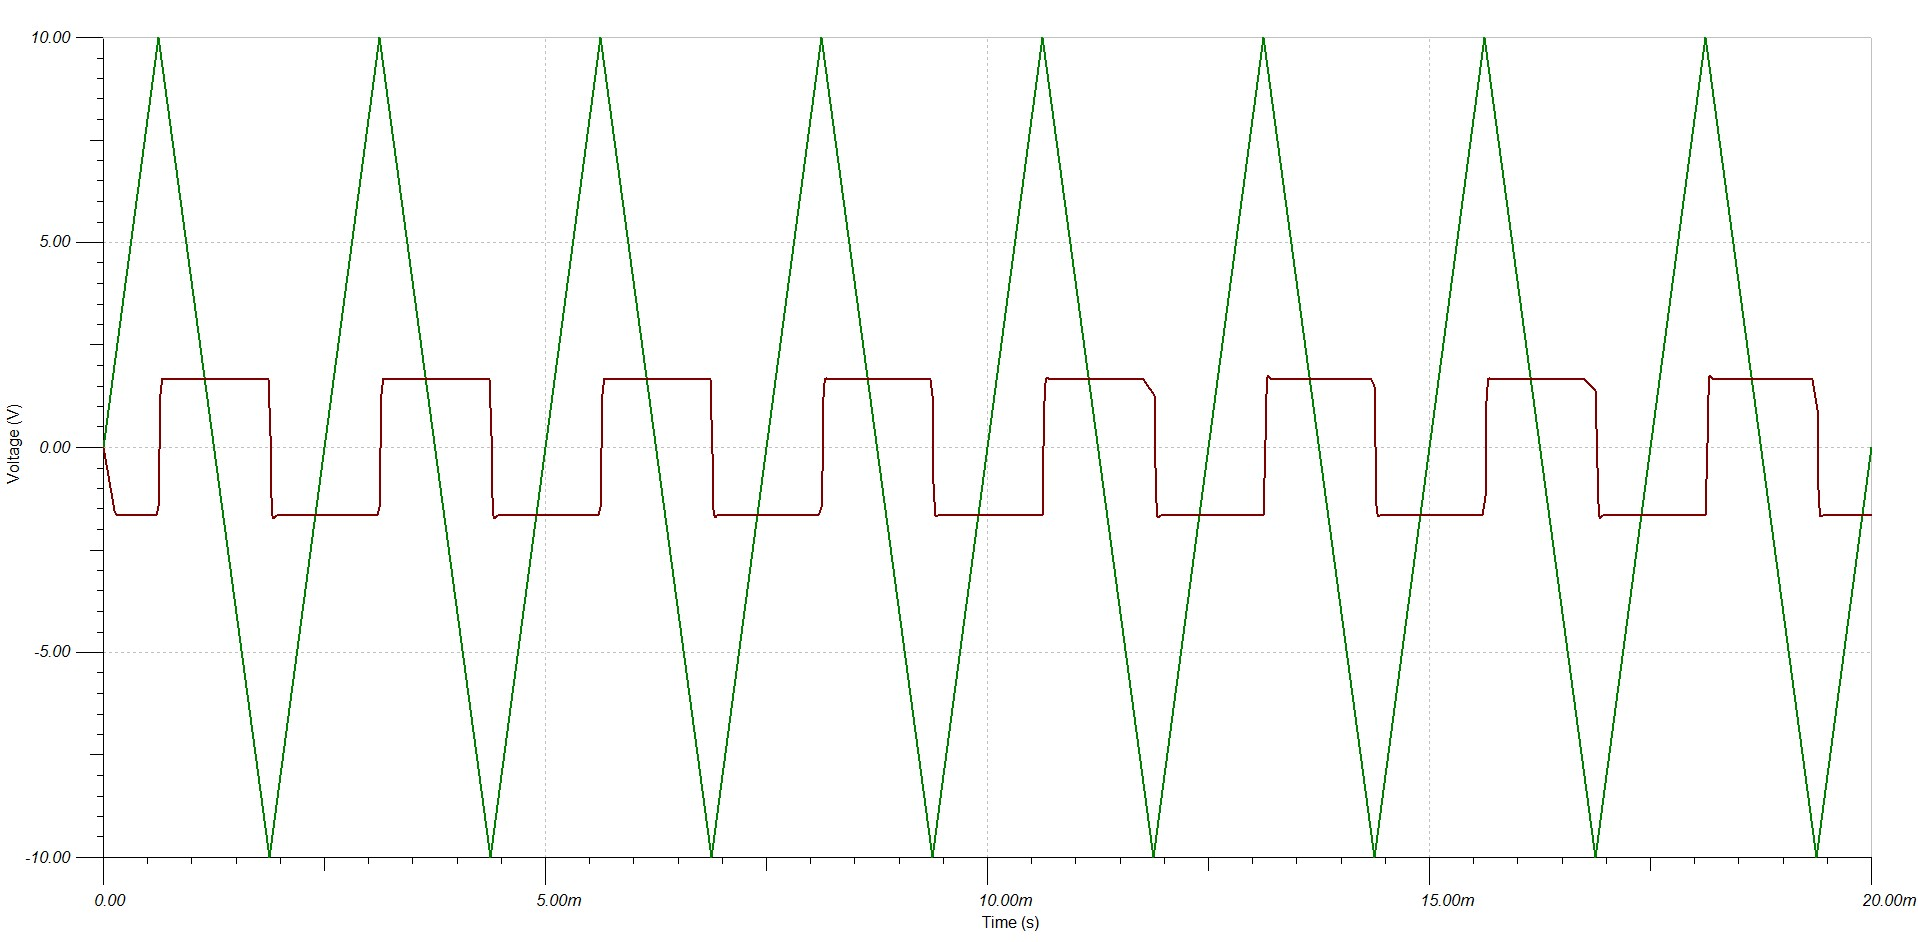
\includegraphics[width=\linewidth]{./res/triang.jpg}
	\caption{Τριγωνικό σήμα.}
\end{figure}

\begin{figure}[H]
	\centering
	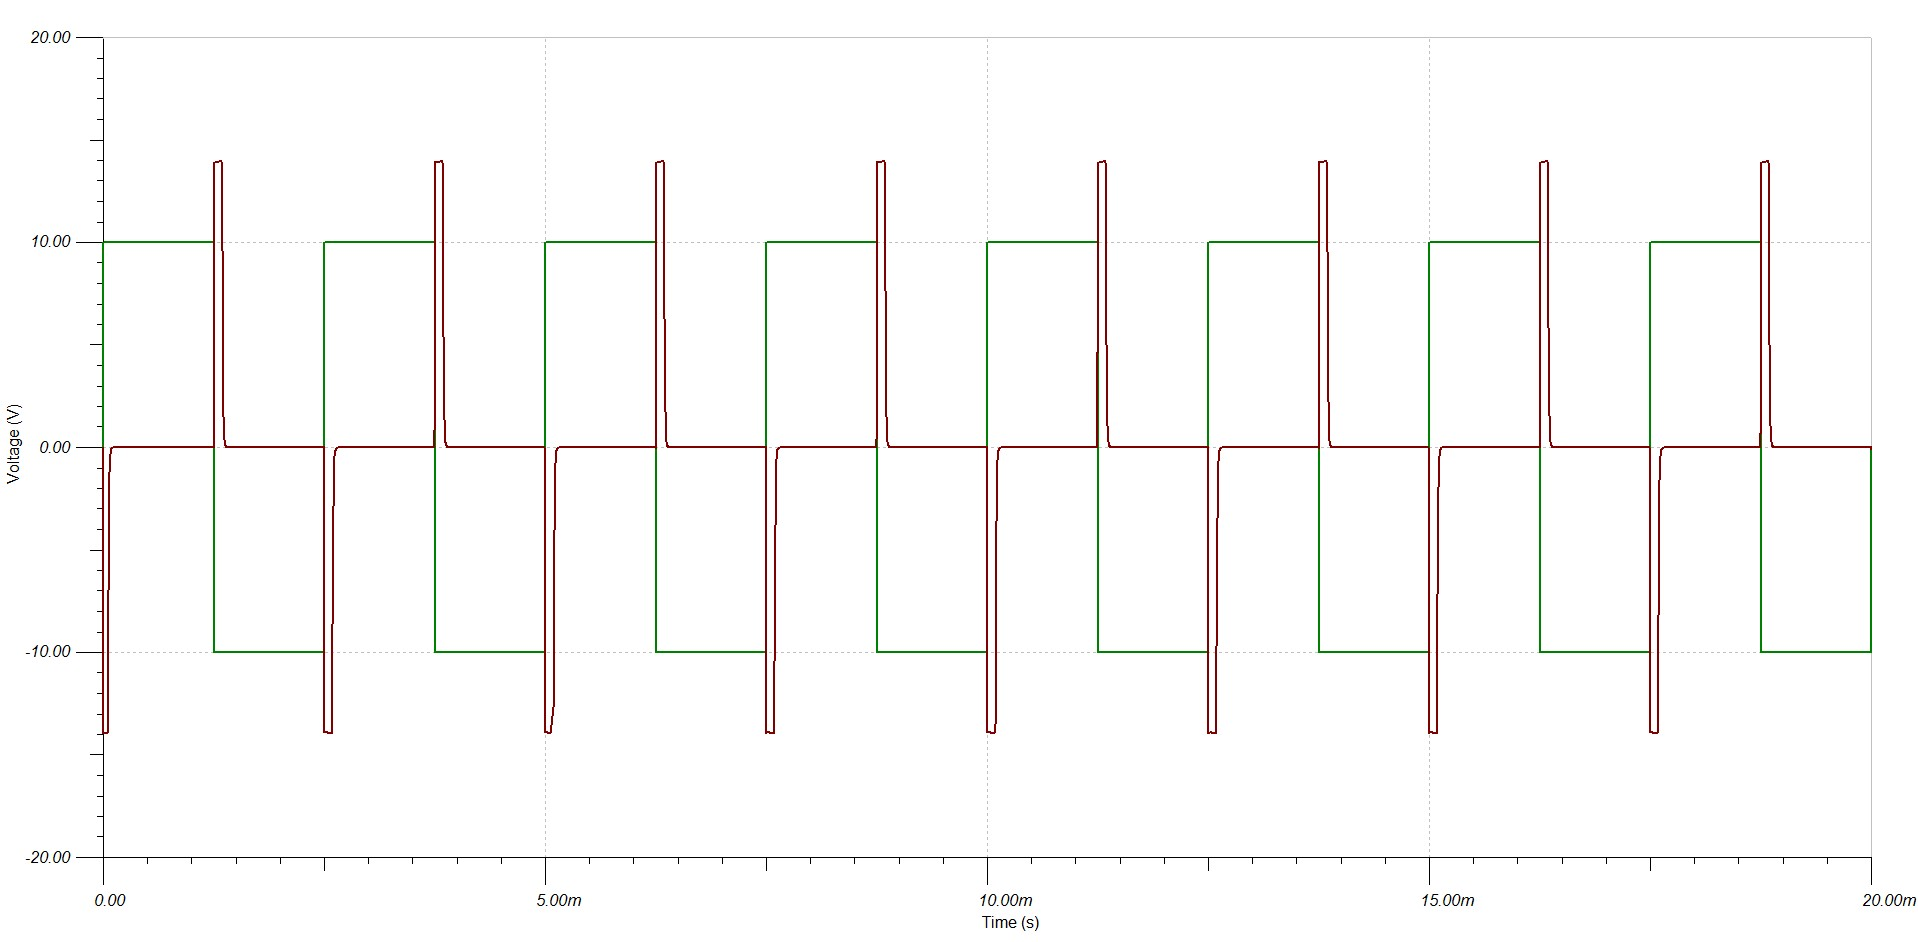
\includegraphics[width=\linewidth]{./res/square.jpg}
	\caption{Τετραγωνικό σήμα.}
\end{figure}

\subsection{Αύξηση τριγωνικής συχνότητας}

\begin{itemize}
	\item Για τριγωνική κυματομορφή εισόδου $7V_{pp}$, $\SI{400}{\hertz}$,
		αρχίστε να αυξάνετε την συχνότητα του σήματος έως ότου να
		παρατηρήσετε στην έξοδο του κυκλώματος την ύπαρξη τριγωνικής
		κυματομορφής (ο διαφοριστής παύει να διαφορίζει και λειτουργεί
		σαν αναστρέφων Τ.Ε). Σημειώστε την πειραματικά μετρούμενη
		συχνότητα του κυκλώματος. Τι σχέση έχει η θεωρητική με την
		πρακτική συχνότητα $F_c$;
\end{itemize}

\begin{figure}[H]
	\centering
	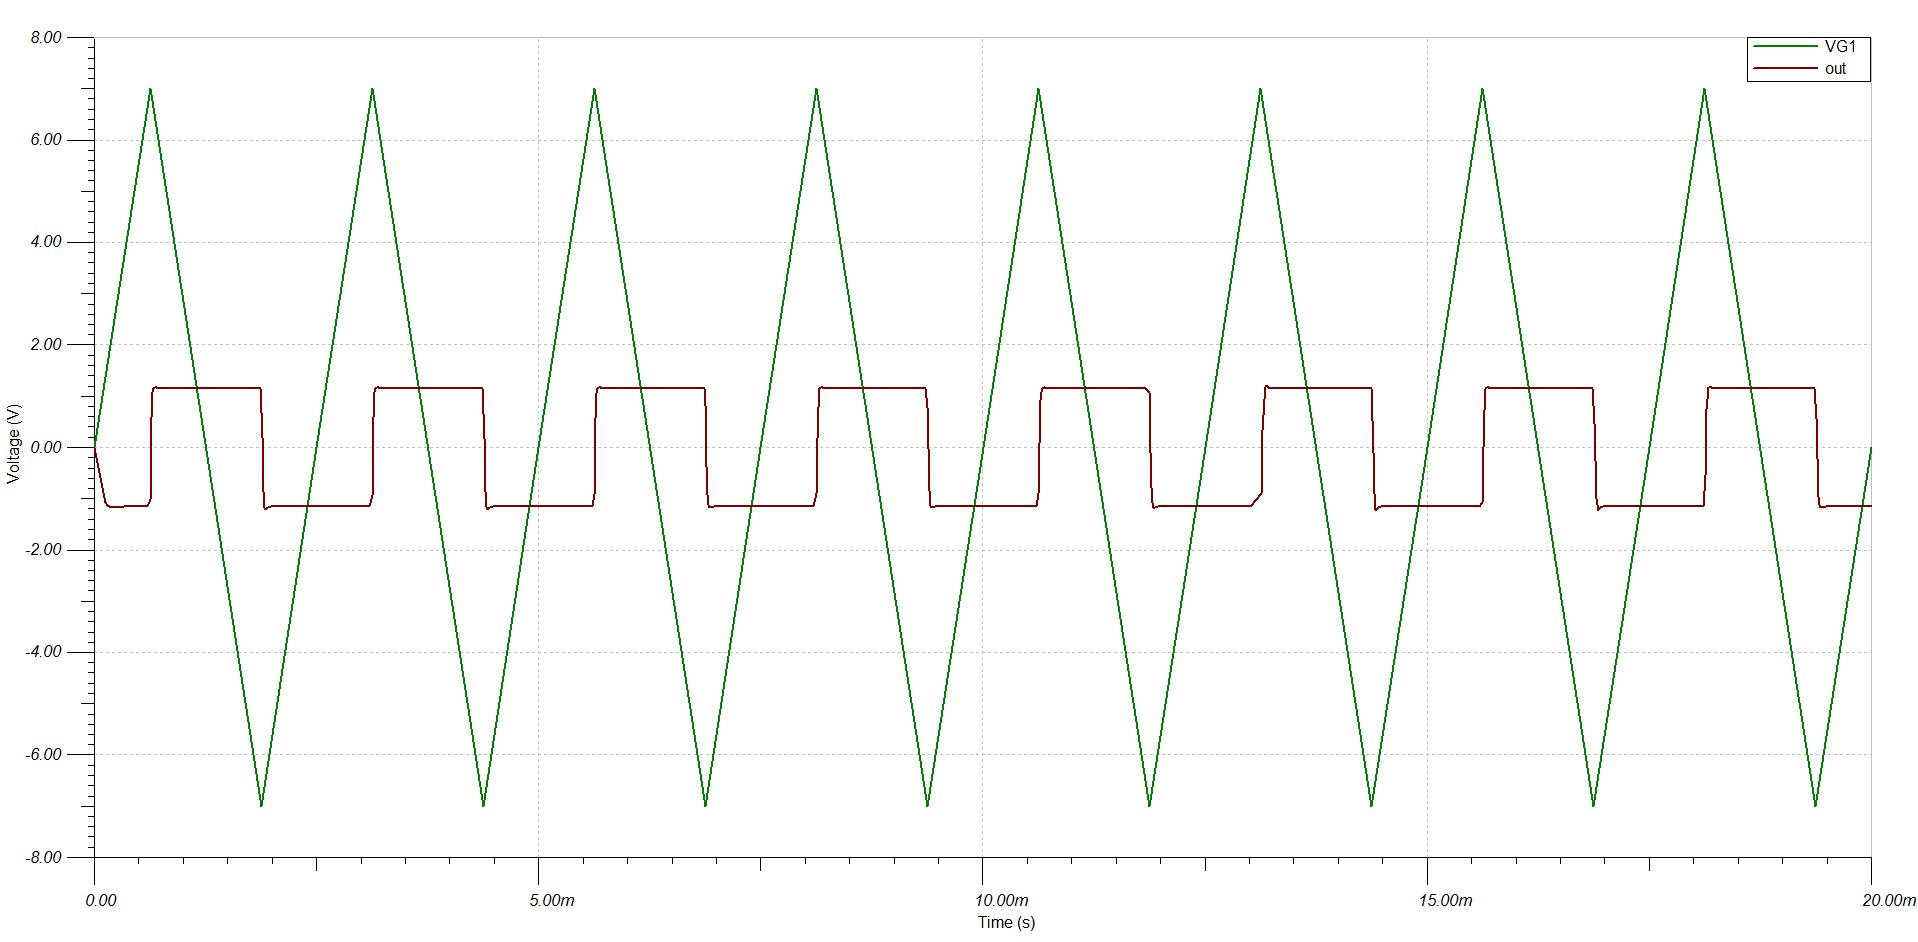
\includegraphics[width=\linewidth]{./res/triang_400hz.jpg}
	\caption{Τριγωνική συχνότητα $\SI{400}{\hertz}$}
\end{figure}

Μετά από πειραματισμό παρατήρησα ότι περίπου στα $\SI{150}{\kilo\hertz}$ η
έξοδος αρχίζει να γίνεται τριγωνικής μορφής, δηλαδή ο διαφοριστής λειτουργεί
σαν αναστρέφων Τ.Ε. Βλέπουμε ότι η πρακτική συχνότητα $\SI{150}{\kilo\hertz}$
είναι πολύ κοντά με την θεωρητική $F_c = \SI{154}{\kilo\hertz}$.

\begin{figure}[H]
	\centering
	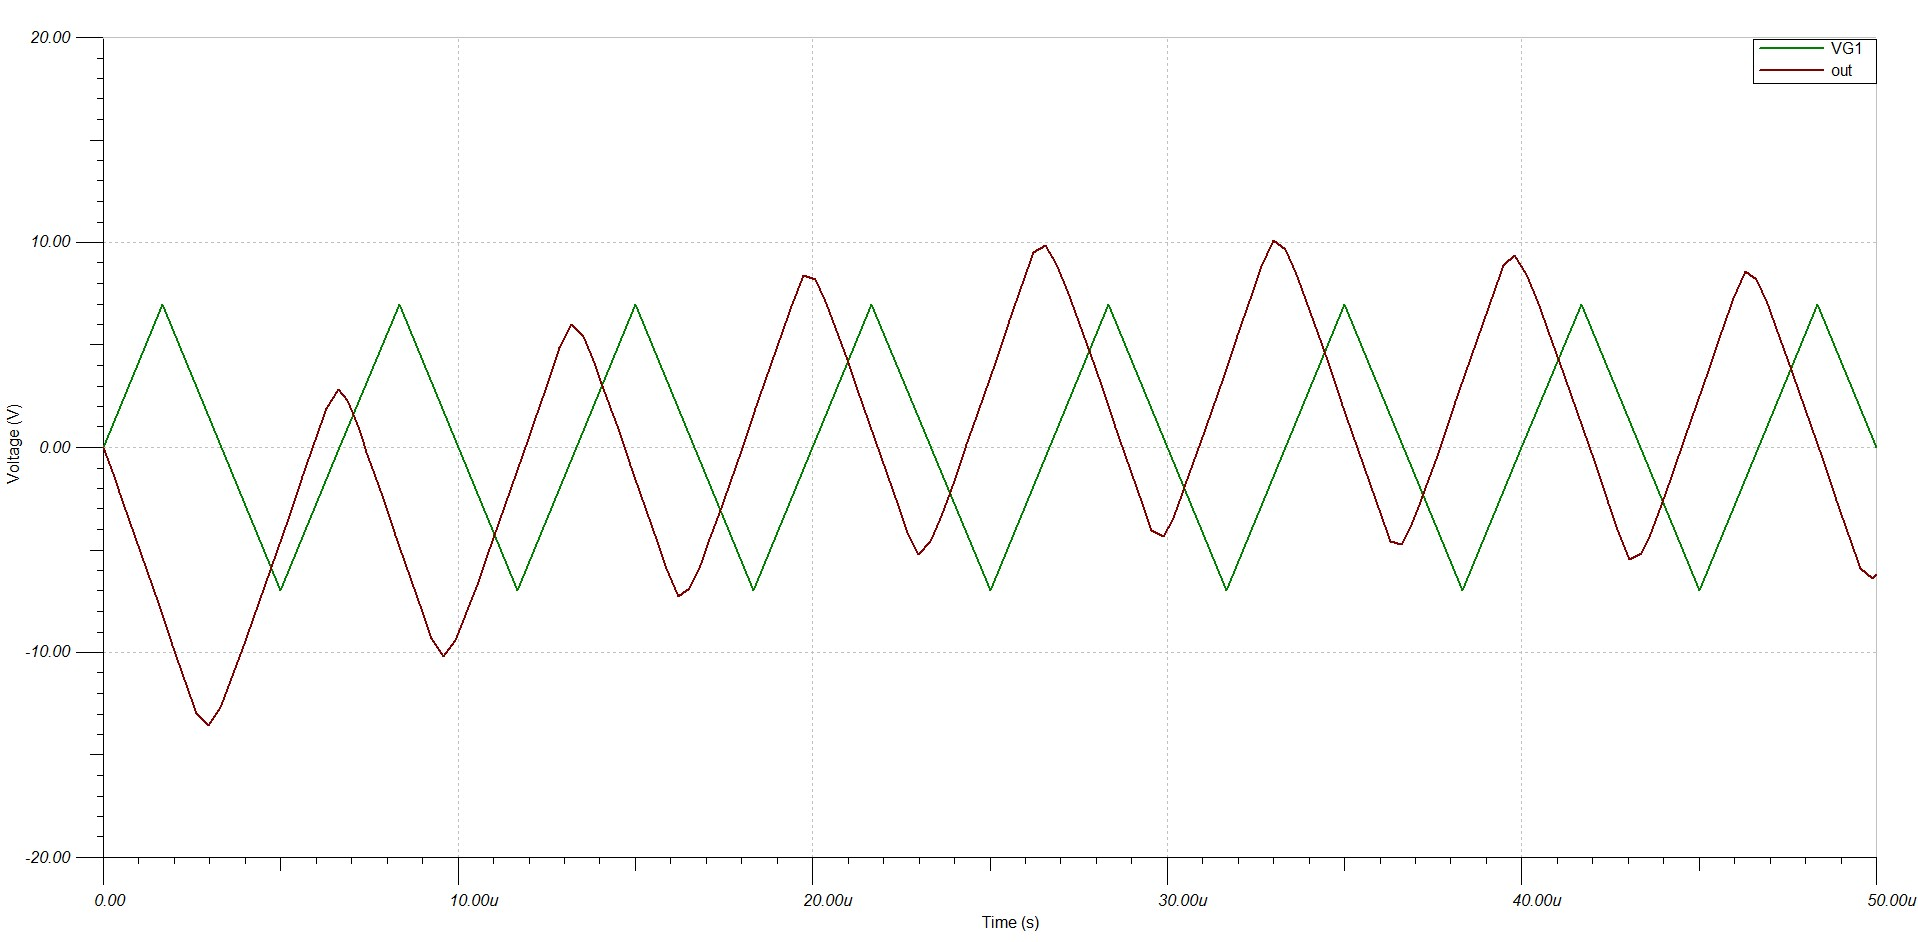
\includegraphics[width=\linewidth]{./res/triang_150khz.jpg}
	\caption{Τριγωνική συχνότητα $\SI{150}{\kilo\hertz}$}
\end{figure}

\section{Breadboard}

Η συνδεσμολογία έγινε στον χώρο του εργαστηρίου. Για την σύνδεση του Τ.Ε
χρησιμοποιούμε το pinout του Τ.Ε:

\begin{figure}[H]
	\centering
	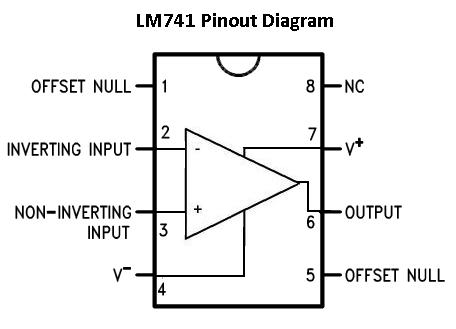
\includegraphics[width=\linewidth]{./res/opamp_pinout.jpg}
	\caption{Pinout Τ.Ε}
\end{figure}

\begin{figure}[H]
	\centering
	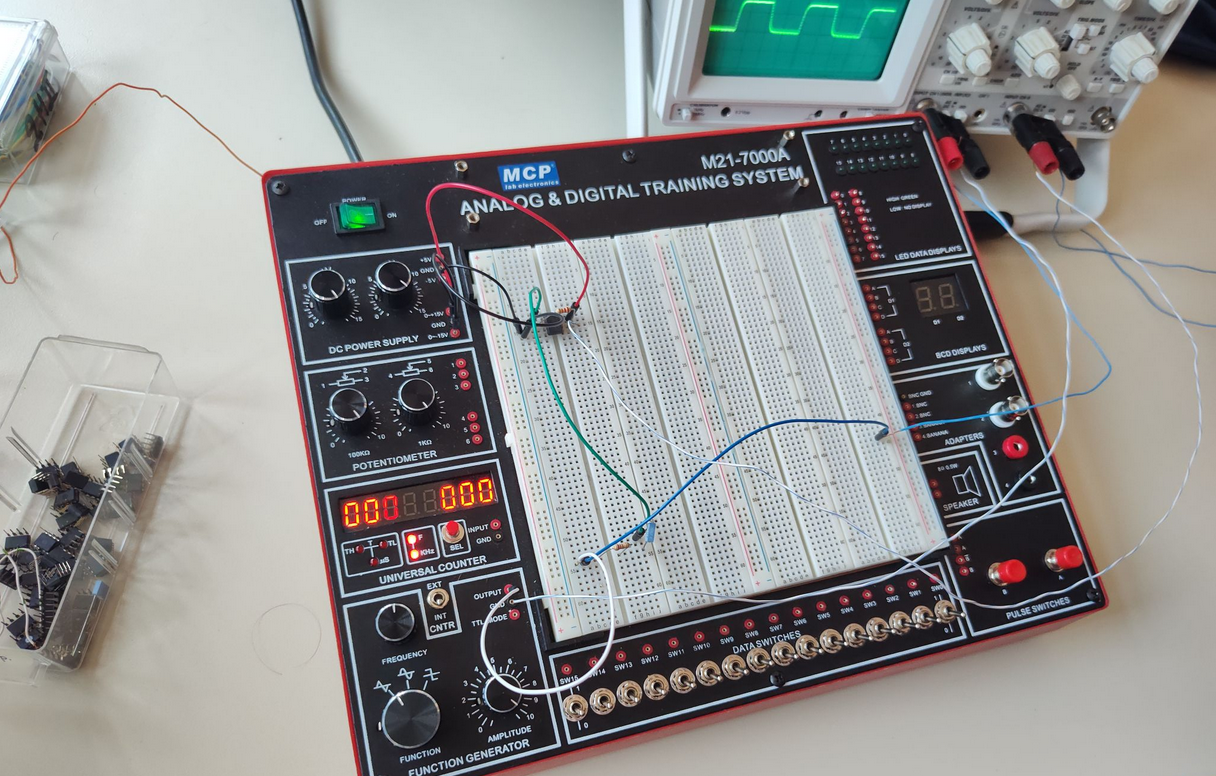
\includegraphics[width=\linewidth]{./res/breadboard.png}
\end{figure}

\end{document}
